\chapter{Integration mit JavaScript}

Im vorherigen Kapitel wurde gezeigt, wie das WebAssembly-Modul erzeugt wird. Grundsätzlich wäre dieses allein theoretisch lauffähig, da aber Interaktion mit JavaScript vorausgesetzt wird (zum Beispiel Objektverwaltung, Konsolenausgaben und native Methoden), ist ein JavaScript-Gerüst rundherum notwendig, das alle Komponenten miteinander verbindet. Daher wird vom Compiler nicht nur ein einfache \lstinline{wasm}-Datei erzeugt, sondern ein Ordner (im Sourcecode \lstinline{Bundle} genannt, nachfolgend auch als "Paket" bezeichnet) mit einigen JavaScript-Dateien und der \lstinline{wasm}-Datei erzeugt.

\section{Aufbau des erzeugten Pakets}

Das Paket hat folgende Ordnerstruktur:
\lstinputlisting{src/javaScriptIntegration/bundleStructure.txt}

Der Name des Wurzelordners ist vom Benutzer der Compilers frei wählbar, daher wurde er hier als Platzhalter mit \lstinline{<bundle-name>} gekennzeichnet. Alle mit einem \lstinline{(*)} gekennzeichnete Dateien sind von den zu kompilierenden Dateien abhängig und werden dynamisch erzeugt. Alle anderen Dateien sind statisch und sind von den zu kompilierenden Dateien unabhängig. Sie werden 1:1 in den Paket-Ordner bei jedem Compileraufruf kopiert.

\subsection{Statische Dateien}

\emph{imports.js} ist für das Erstellen des Import-Objekts verantwortlich, das beim Instanzieren des WebAssembly-Moduls benötigt wird. Hier werden die JavaScript-Implementie\-rungen von sprachinternen Funktionalitäten, als auch die JavaScript-Pendants nativer Methoden in ein Objekt zusammengefasst.

\emph{internal.js} enthält die JavaScript-Implementierungen von sprachinternen Funktionalitäten für Arrays und Stringkonkatenationen.

\emph{runtime.js} definiert die Laufzeitumgebung für das Zusammenspiel zwischen JavaScript und WebAssembly/MiniJava. Hier befindet sich die Objektverwaltung und diverse Hilfsfunktionen um Daten zwischen JavaScript und WebAssembly/MiniJava auszutauschen und um von JavaScript ausgehend MiniJava-Methoden aufrufen zu können.

\subsection{Dynamische Dateien}

Alle JavaScript-Pendants für native Methoden werden in den Ordner \emph{native} kopiert. Um dabei potenzielle Dateinamenkollisionen zu umgehen, werden alle Dateien ab 0 beginnend nummeriert.

Der generierte Bytecode wird in der Datei \emph{module.wasm} abgelegt. Als Zwischenprodukt entsteht beim Kompilieren die Datei \emph{module.wat}, die lediglich die textuelle Repräsentation des WebAssembly-Moduls ist\footnote{Dies hat den Hintergrund, dass das Erstellen der textuellen Repräsentation wesentlich einfacher ist. Außerdem können beim Entwickeln des Compilers potenzielle Fehler leichter in einer Textdatei als in einer binäaren Datei gefunden werden.}. Aus dieser Datei entsteht mit dem Werkzeug \lstinline{wat2wasm}\cite{WABT} dann die binäre Form des Moduls. Die textuelle Repräsentation wird zur Laufzeit grundsätzlich nicht benötigt.

Alle im MiniJava-Sourcecode vorhandenen Stringliterale werden in der Datei \emph{module.js} registriert. Außerdem werden zur Compile-Zeit sämtliche Konstrukturen, Getter und Setter für MiniJava-Klassen generiert und in dieser Datei gespeichert. Weiters referenziert diese Datei alle JavaScript-Dateien im Ordner \emph{native}.

\subsection{Zusammenhang zwischen den Dateien}

Je nachdem, auf welcher Plattform das Paket ausgeführt wird, muss das WebAssembly-Modul unterschiedlich geladen werden: Bei Node.js kann das Modul direkt aus dem Dateisystem gelesen werden, im Browser muss es von einem Web-Server heruntergeladen werden. Um dem Benutzer des Pakets hier Flexibilität zu ermöglichen, wird das WebAssembly-Modul nicht direkt von den anderen JavaScript-Dateien referenziert.

In der folgenden Grafik wird der Zusammenhang zwischen den JavaScript-Dateien visualisiert:

\begin{center}
    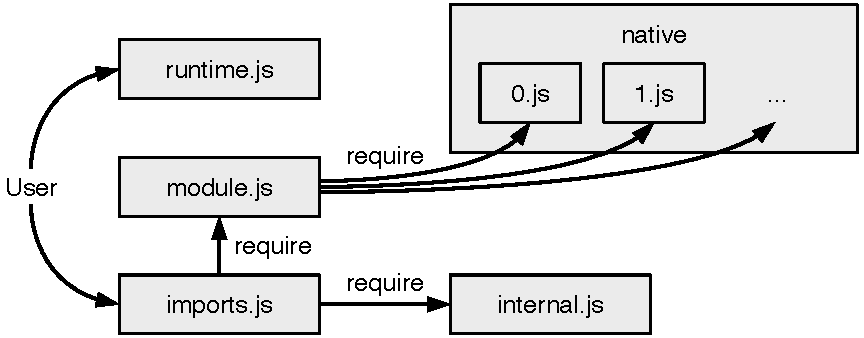
\includegraphics[width=0.8\textwidth]{javaScriptIntegration/bundle}
\end{center}

Auf die praktische Verwendung des gesamten Pakets wird in diesem Kapitel nicht eingangen. Im Abschnitt \ref{sec:NodeJSExample} wird anhand eines Beispiels gezeigt, wie sich das Paket in eine Node.js-Konsolenanwendung integrieren lässt.

\section{JavaScript-Codegenerierung}

Wie im vorherigen Abschnitt beschrieben, wird beim Kompilieren JavaScript-Code in der Datei \emph{module.js} generiert.

Beim Erzeugen des Bytecodes wurden bereits für die Stringliterale Speicheradressen (ab 1 beginnend) festgelegt. Daher müssen später zur Laufzeit die Stringliterale in der Reihenfolge der zuvor zugewiesenen Speicheradressen (siehe Abschnitt TODO) registriert werden. Dies muss geschehen, bevor das WebAssembly-Modul gestartet wird, da zu diesem Zeitpunkt noch keine Objekte erstellt wurden. So wird garantiert, dass sich die Adressen nicht verschieben.

Außerdem muss für jede Klasse ein Konstruktur generiert werden. Dieser hat die Aufgabe, ein JavaScript-Objekt zu erzeugen, in dem alle Instanzvariablen mit einem (je nach Datentyp) sinnvollen Platzhalterwert initialisiert werden. Außerdem wird der MiniJava-Datentyp mit dem Objekt verknüpft. Die Konstrukturen geben als Rückgabewert die Adresse des erzeugen Objekts zurück.

Instanzvariablen von MiniJava-Klassen werden direkt auf Instanzvariablen von Java\-Script-Objekten abgebildet. Da WebAssembly nicht direkt auf JavaScript-Objekte zugreifen kann, müssen für diese Getter und Setter erzeugt werden, die diese Aufgabe übernehmen. Die Getter bekommen als Parameter nur die Adresse bzw. Referenz des Objekts und müssen den Wert der Instanzvariable (oder die Adresse wenn die Instanzvariable ein Objekt referenziert) zurückgeben. Ähnlich funktionieren die Setter: Diese bekommen zwei Parameter, die Adresse des Objekts und den Wert des neuen Werts für die Instanzvariable (oder die Adresse, wenn es sich um referenzierte Objekte handelt). Setter haben keinen Rückgabewert.

Die Codegenerierung wird anhand eines überschaubaren Beispiel nun detailliert gezeigt. Nachfolgend sieht man den MiniJava-Code für dieses Beispiel:

\lstinputlisting{src/javaScriptIntegration/Example.minijava}

Aus diesem Code wurde die Datei \emph{module.js} erzeugt:

\lstinputlisting{src/javaScriptIntegration/module.js}

Man sieht am Beginn die zwei Stringliterale (1). Etwas weiter unten ist der Konstruktor, der die Instanzvariablen mit \lstinline{0} und \lstinline{null} initialisiert (2). Bei (3) werden Getter und Setter für die \lstinline{int}-Instanzvariable definiert. Da es sich um einen elementaren Datentyp handelt, kann der Wert direkt aus dem übergebenen Parameter gelesen werden (Setter) bzw. als Rückgabewert zurückgegeben werden (Getter). Beim Getter und Setter für die \lstinline{String}-Instanzvarible (4) muss der Parameter beim Setter zunächst derefenziert werden bzw. muss beim Getter zunächst eine Referenz auf das Objekt erzeugt werden.

\section{Objektverwaltung für MiniJava in JavaScript}

Sämtliche Objekte, auf die von MiniJava zugegriffen wird, werden in JavaScript als "echte" JavaScript-Objekte verwaltet. Diese Objekte werden in MiniJava über eine Adresse bzw. Referenz angesprochen. Im Wesentlichen entspricht diese Referenz einer fortlaufenden Nummer, die bei 1 beginnt, da 0 \lstinline{null} entspricht.

Es muss möglich sein, eindeutig von einem Objekt auf die Referenz und umgekehrt schließen zu können. Für beide Richtungen wird diese Abbildung jeweils in einer Java\-Script-\lstinline{Map} gespeichert.

Diese Datenstrukturen werden in der JavaScript-Klasse \lstinline{Runtime} verwaltet. Im Konstruktor werden diese sinnvoll initialisiert, beispielsweise wird die Referenz 0 auf \lstinline{null} und umgekehrt abgebildet:

\lstinputlisting{src/javaScriptIntegration/runtimeConstructor.js}

Weiters werden drei Methoden zur Verfügung gestellt, die das Erstellen einer Referenz auf ein JavaScript-Objekt und das Dereferenzieren einer Referenz kapseln:

\lstinputlisting{src/javaScriptIntegration/runtimeRefs.js}

Die Methode \lstinline{wasmRefType} sollte genau dann verwendet werden, wenn das erste Mal eine Referenz für ein JavaScript-Objekt angefordert wird, da hier der MiniJava-Datentyp des Objekts registriert wird. Dieser Typ wird später für Methodenaufrufe benötigt.

Wie der Name der Methoden bereits erahnen lässt, liefert \lstinline{wasmDeref} das Objekt bzw. \lstinline{null} hinter der Referenz. \lstinline{wasmRef} liefert die Referenz auf das Objekt, falls bereits eine Referenz erstellt wurde oder erstellt eine neue, falls das Objekt noch keine Referenz besitzt.

\section{Hilfsfunktionen}

Die Klasse \lstinline{Runtime} bietet noch einige nützliche Hilfsmethoden an, die das Zusammenspiel zwischen JavaScript und WebAssembly/MiniJava erleichtern sollen:

\lstinputlisting{src/javaScriptIntegration/runtimeHelpers.js}

Mit \lstinline{wasmBoolean} kann ein MiniJava-\lstinline{boolean} (entspricht einer Ganzahl in WebAssembly) in einen JavaScript-\lstinline{boolean} konvertiert werden. In die andere Richtung ist keine explizite Konvertierung erforderlich.

Mit \lstinline{charToWasm} und \lstinline{wasmToChar} kann zwischen einem MiniJava-\lstinline{char} (entspricht ebenfalls einer Ganzzahl in WebAssembly) und einem JavaScript-\lstinline{string} mit genau einem Zeichen konvertiert werden.
Es musste ein JavaScript-\lstinline{string} verwendet werden, da JavaScript keinen eigenen Datentyp für einzelne Zeichen besitzt.

\section{Sprachinterne Funktionalitäten}

MiniJava bietet einige Sprachfeatures an, die nicht zur Gänze in WebAssembly abgebildet werden können, da sie mit JavaScript-Objekten interagieren. Dazu zählen alle Funktionalitäten rund um Arrays wie das Erstellen eines Arrays, das Abfragen der Länge des Arrays und das Lesen und Schreiben über einen Index. Außerdem bietet MiniJava das Konkatenieren von Strings mit diversen Datentypen an.

\subsection{Arrayfunktionen}

Die Implementierung der Arrayfunktionen sind vom konkreten Element-Datentyp des Arrays abhängig. Allgemein lassen sich daher vier Fälle unterscheiden:

\begin{description}
    \item[Werte numerische Datentypen] wie \lstinline{int} und \lstinline{float} werden auf denselben JavaScript-Daten\-typ abgebildet, da JavaScript nur den Datentyp \lstinline{number} kennt.
    \item[boolean-Werte] müssen zwischen JavaScripts \lstinline{true} und \lstinline{false} auf 1 und 0 und umgekehrt abgebildet werden, da WebAssembly keinen eigenen Datentyp für Wahrheitswerte besitzt
    \item[char-Werte] müssen zwischen einer Ganzzahl und einem String mit einem Zeichen abgebildet werden.
    \item[Objekte] müssen auf Referenzen und umgekehrt abgebildet werden. 
\end{description}

Sämtliche Funktionen für Arrays wurden für diese vier Fälle einzeln implmentiert und funktionieren konzeptionell ähnlich. Im WebAssembly-Modul werden die Funktionen über einen Funktionsnamen importiert, der diesem Schema entspricht: \lstinline{<function>_array_<type>}.

Am interessantesten sind die Funktionen für Arrays von Objekten, daher werden diese nun im Detail betrachtet.

Beim Erstellen eines Arrays wird ein JavaScript-Array in der angeforderten Größe erstellt und mit Standardwerten (hier \lstinline{null}) vorbefüllt:
\lstinputlisting{src/javaScriptIntegration/arrayNew.js}

Das Abrufen eines Objekts über den Index funktioniert folgendermaßen, dabei muss zunächst das Array selbst derefenziert werden. Anschließend wird für das über den Index erhaltene Objekt mit \lstinline{runtime.wasmRef} eine Referenz erstellt:
\lstinputlisting{src/javaScriptIntegration/arrayGet.js}

Analog dazu funktioniert das Setzen eines Objekts an einem Index:
\lstinputlisting{src/javaScriptIntegration/arraySet.js}

Die Funktion für das Abfragen der Länge des Arrays ist typunabhängig, daher gibt hier nur eine Implementierung:

\lstinputlisting{src/javaScriptIntegration/arrayLength.js}

\subsection{Stringkonkatenation}

Alle Verwendungen des MiniJava-Konkatenationsoperators \lstinline{+} werden auf JavaScript-Funktionen abgebildet. Dabei muss zumindest auf einer Seite des Operators ein String stehen. Abhängig vom Datentyp "auf der anderen Seite" gibt es (ähnlich wie bei den Arrays) eine eigene Implementierung. Im WebAssembly-Modul werden die Funktionen über einen Funktionsnamen importiert, der diesem Schema entspricht: \lstinline{+_<left-type>_<right-type>}.

Die einfachste Variante ist das Konkatenieren von zwei Strings. Hier werden zunächst die Referenzen der beiden Strings dereferenziert. Anschließend wird eine Referenz auf den zusammengesetzten String erstellt:
\lstinputlisting{src/javaScriptIntegration/stringString.js}

Ähnlich wie bei den Arrays gibt es dieselben vier Fälle für die Datentypen "auf der anderen Seite". Für jeden Fall gibt es zwei Varianten: Datentyp auf der linken Seite und String auf der rechten Seite sowie String auf der linken Seite und Datentyp auf der rechten Seite. Somit ergibt das insgesamt acht Funktionen.

Da das Konkatenieren für die einzelnen Datentypen konzeptionell ähnlich funktioniert, werden stellvertretend nun beispielhaft die zwei Funktionen gezeigt, um einen String mit einem numerischen Wert zu verketten:
\lstinputlisting{src/javaScriptIntegration/stringNumeric.js}

\section{Methodenaufrufe von JavaScript nach MiniJava}

Alle MiniJava-Methoden, die mit dem Schlüsselwort \lstinline{public} gekennzeichnet wurden, werden als Funktion im WebAssembly-Modul exportiert. Dabei wird dieselbe Benennungskonvention wie für das Importieren von nativen Methoden verwendet (siehe Abschnitt TODO).

In der JavaScript-Klasse \lstinline{Runtime} wird die Funktion \lstinline{findMethod} zur Verfügung gestellt, mit der aus Klassenname, Methodenname und der Eingabeparametertypliste der Methodenname zusammengebaut wird. Anschließend wird die Funktion aus der \lstinline{exports}-Datenstruktur der WebAssembly-Modulinstanz abgerufen.

\lstinputlisting{src/javaScriptIntegration/runtimeFindMethod.js}

Auf dieser Funktion aufbauend können nun Aufrufe auf statische Methoden und Instanzmethoden realisiert werden.

\subsection{Statische Methodenaufrufe}

Bei statischen Aufrufen kann \lstinline{findMethod} praktisch direkt verwendet werden. Um dem Verwender der \lstinline{Runtime}-Klasse eine einheitliche Schnittstelle zu bieten, wird der Aufruf von \lstinline{findMethod} in der Methode \lstinline{staticMethod} gekapselt:

\lstinputlisting{src/javaScriptIntegration/runtimeStaticMethod.js}

Nun kann ein statischer Aufruf durchgeführt werden. So wird beispielsweise die Mini\-Java-Methode \lstinline{public static int add(int a, int b)} der MiniJava-Klasse \lstinline{Utils} in Java\-Script mit den Parametern \lstinline{a = 3} und \lstinline{b = 4} aufgerufen:

\lstinputlisting{src/javaScriptIntegration/staticCall.js}

\subsection{Instanzmethodenaufrufe}

Instanzmethoden können nicht direkt wie statische Methoden aufgerufen werden, da zunächst der Typ des Objekts, auf das die Methode aufgerufen wird, bestimmt werden muss. Damit dies möglich ist, muss das Empfängerobjekt bereits mit \lstinline{runtime.wasmRefType} registriert sein. Anschließend kann mit \lstinline{findMethod} die Methode gesucht werden. Da Instanzmethoden per Konvention als ersten Parameter eine Referenz auf das Empfängerobjekt erwarten ("\lstinline{this}-Referenz", siehe Abschnitt TODO), muss die Referenz als erster Parameter beim Aufruf eingefügt werden:

\lstinputlisting{src/javaScriptIntegration/runtimeInstanceMethod.js}

Da die Anzahl der Parameter von der tatsächlichen Methode abhängig ist, werden in Zeile 4 beim Lambda-Ausdruck in der Parameterliste "Rest-Parameter" (\lstinline{...args}) \cite{MDNJavaScript} verwendet, die alle übergebenen Parameter in der Liste \lstinline{args} speichern. Beim Aufruf der WebAssembly-Funktion muss diese Parameterliste wieder "ausgepackt" werden - ansonsten würde man ja die Parameterliste als ein Listenobjekt übergeben. Dafür wird die "Spread-Syntax" (\lstinline{...args}) verwendet. Die beiden Konstrukte sehen syntaktisch ident aus, erfüllen aber die jeweils gegensätzliche Funktion.

Nun kann ein Aufruf einer Instanzmethode durchgeführt werden. So wird beispielsweise die MiniJava-Methode \lstinline{public void increment(int a)} eines Objekts \lstinline{obj} in JavaScript mit dem Parameter \lstinline{a = 3} aufgerufen:

\lstinputlisting{src/javaScriptIntegration/instanceCall.js}

\section{Standardbibliothek}

Jede Programmiersprache benötigt eine Standardbibliothek. Diese sollte einerseits Basisfunktionalitäten zur Verfügung stellen, um sinnvoll mit der Laufzeitumgebung interagieren zu können. Andererseits können hier oft verwendete Basisfunktionalitäten zur Verfügung gestellt werden, die in nahezu jeder Anwendung benötigt werden.

Um einen Eindruck zu vermitteln, wie man für MiniJava die Grundsteine für eine Standardbibliothek legen könnte, wurden einige solche Basisfunktionalitäten implementiert. In diesem Abschnitt werden einige Ausschnitte daraus präsentiert.

Bei Interaktionen mit der Laufzeitumgebung sind native Methoden mit JavaScript-Pendants unumgänglich. Somit vermittelt dieser Abschnitt ebenfalls einen Einblick, wie native Methoden aufgebaut werden können.

\subsection{Konsolenausgabe}
Die einfachste Form einer Benutzeroberfläche ist die Konsole. Daher ist die Konsole die absolute Grundvoraussetzung, um die Ergebnisse eigener Programme sehen zu können.

Sämtliche Funktionalitäten für die Konsolenausgabe wurden in der MiniJava-Klasse \lstinline{Console} gekapselt, die eine Reihe an statischen Methoden zur Verfügung stellt. Hier werden nur zwei davon gezeigt, in der vollständigen Implementierung sind noch einige mehr vorhanden, wie zum Beispiel zur Ausgabe von Arrays.

In MiniJava werden die Methoden folgendermaßen definiert:
\lstinputlisting{src/javaScriptIntegration/Console.minijava}

In JavaScript werden die Aufrufe an \lstinline{console.log} delegiert:
\lstinputlisting{src/javaScriptIntegration/Console.js}

\subsection{Methoden für Strings}

Strings gehören ebenso zum Grundwerkzeug beim Programmieren dazu. Zu den Basisfunktionalitäten für Strings zählen das Bestimmen der Länge, das Abfragen eines Zeichens an einer Stelle und das Vergleichen, ob zwei Strings gleich sind.

Diese drei Funktionalitäten werden als Instanzmethoden in der MiniJava-Klasse \lstinline{String} definiert:
\lstinputlisting{src/javaScriptIntegration/String.minijava}

In JavaScript werden diese mit Hilfe von bereits bestehenden Funktionalität implementiert:
\lstinputlisting{src/javaScriptIntegration/String.js}

\subsection{Konvertieren zwischen Ganzzahlen und Strings}

Oft werden in Benutzereingaben Zahlen erfasst. Diese stehen dann in Form eines Strings zur Verfügung. Um mit den Werten sinnvoll arbeiten zu können, müssen die Strings in eine Zahl konvertiert werden. Umgekehrt müssen Zahlen für zum Beispiel Ausgaben wiederum in Strings konvertiert werden.

Dafür wurden (angelehnt an die echte Java-Standardbibliothek) zwei statische Methoden in der MiniJava-Klasse \lstinline{Integer} definiert:
\lstinputlisting{src/javaScriptIntegration/Integer.minijava}

Da JavaScript auch hier bereits Funktionalitäten zur Verfügung stellt, wird das Konvertieren an JavaScript delegiert:
\lstinputlisting{src/javaScriptIntegration/Integer.js}
